\documentclass{article}
\usepackage[utf8]{inputenc}
\usepackage[brazil]{babel}
\usepackage{epsfig}
\usepackage{fancyhdr}
\usepackage{indentfirst} %In­dent first para­graph af­ter sec­tion header
\usepackage{titlesec}
\usepackage{amsmath}
\usepackage{amsthm}
\usepackage{listings}
\usepackage{color}
\usepackage[table,xcdraw]{xcolor}

\pagestyle{empty}

\headheight 40mm      %
\oddsidemargin 2.0mm  %
\evensidemargin 2.0mm %
\topmargin -40mm      %
\textheight 250mm     %
\textwidth 160mm      %
%
\newcounter{execs}
\setcounter{execs}{0}
\newcommand{\exec}[0]{\addtocounter{execs}{1}\item[\textbf{\arabic{execs}.}]}

\fancypagestyle{first}
{
\pagestyle{fancy}
}
%%%%%%%%%%%%%%%%%%%%%%%%%%%%%%%%%%%%%%%%%%%%%%%%%%%%%%%%
%%%%%%%%%%%%%%%%%%%%%%%%%%%%%%%%%%%%%%%%%%%%%%%%%%%%%%%%
% PLEASE, EDIT THIS!
\fancyhead[LO]{\small $4^a$ Lista \\ 
                DCC008 - Cálculo Numérico  \\
                \textbf{Entrega: 28 de Outubro de 2018} }

\fancyhead[RO]{\small Universidade Federal de Juiz de Fora - UFJF \\ 
                Departamento de Ciência da Computação \\
               \textit{Nome: Aluno 1}\\
               \textit{Nome: Aluno 2}}


\begin{document}
\thispagestyle{first}
\noindent \textbf{Obs1.:}  Escolha um ou mais métodos de interpolação dado em aula para resolver os problemas abaixo.

\noindent \textbf{Obs2.:}  Discuta os resultados.

\begin{itemize}

\exec Considere a função
$$
f(x)=\dfrac{1}{1+25x^2}
$$
definida no intervalo $x\in [a,b]$ com $a=-1$ e $b=1$. 

\begin{itemize}

\item[a)] Seja $P_n(x)$ o polinômio que interpola $f(x)$ nos pontos
$$
x_k = a + \dfrac{b-a}{n}k, \quad k = 0,1,2,...,n
$$
igualmente espaçados no intervalo $[a,b]$. Nesse contexto,
apresente gráficos comparando $P_n(x)$ com $f(x)$ para $n= 2,3,4,5,6,7,8,9,10$.

\item [b)] Repita o item (a), porém utilizando os pontos
$$
x_k = \dfrac{a+b}{2} - \dfrac{b-a}{2}\cos\left(\dfrac{k}{n}\pi \right), \quad k = 0,1,2,...,n.
$$
igualmente espaçados no intervalo $[a,b]$.
\item [c)] Repita o item (a), considerando  uma interpolação \textbf{linear por partes} com nós
$$
x_k = -1 + \dfrac{2}{n}k, \quad k = 0,1,2,...,n.
$$
igualmente espaçados no intervalo $[a,b]$.

\item [d)] Calcule o erro de interpolação na norma do máximo $\|f(x)-P_n(x)\|_{\infty} $ e construa uma tabela comparando os resultados obtidos nos itens (a), (b) e (c) para $n = 2,5,10$. Comente os resultados.
%$$
%\|f(x)-P_n(x)\| = \sqrt{\int_a^b |f(x)-P_n(x)|^2}
%$$
%\textbf{obs.:} Para o caso da interpolação linear por partes, calcule o erro de cada intervalo, separadamente, e some os resultados.

\end{itemize}

\end{itemize}

Para a resolução da Lista 4 foi escolhido o método de interpolação de Lagrande, através de sua analise foram obtidos os seguintes resultados;

\newpage
\text Para a resolução da interpolação do item a:

\begin{figure}[!htb]
\centering
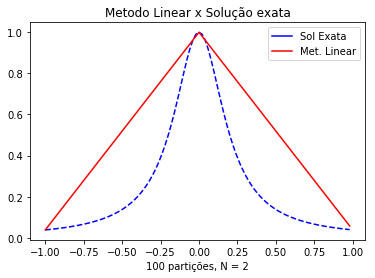
\includegraphics [width=5cm,height=5cm]{LSEa2.png}
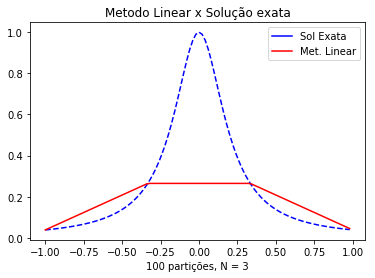
\includegraphics [width=5cm,height=5cm]{LSEa3.png}
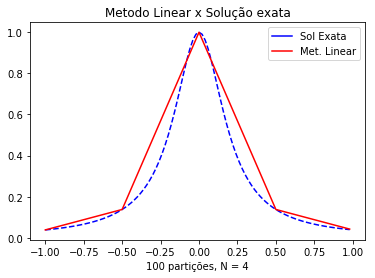
\includegraphics [width=5cm,height=5cm]{LSEa4.png}
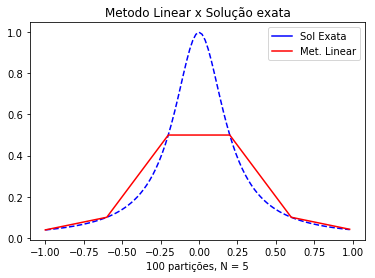
\includegraphics [width=5cm,height=5cm]{LSEa5.png}
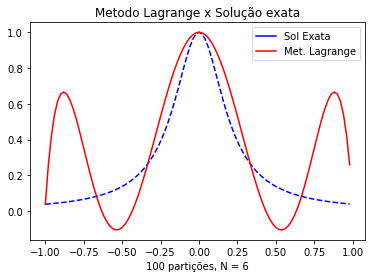
\includegraphics [width=5cm,height=5cm]{LSEa6.png}
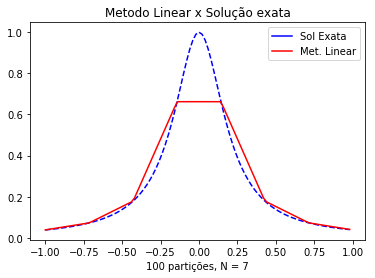
\includegraphics [width=5cm,height=5cm]{LSEa7.png}
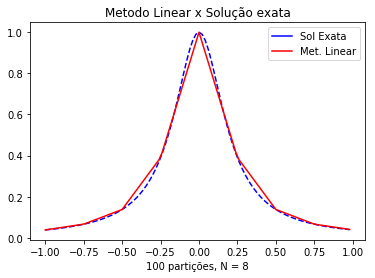
\includegraphics [width=5cm,height=5cm]{LSEa8.png}
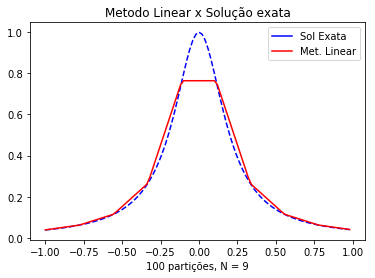
\includegraphics [width=5cm,height=5cm]{LSEa9.png}
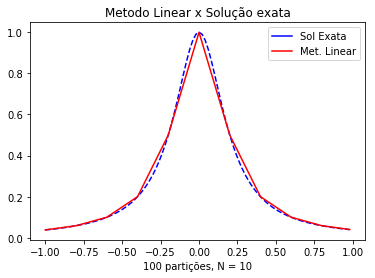
\includegraphics [width=5cm,height=5cm]{LSEa10.png}
\end{figure}

\newpage

\text Seguindo a Solução Exata x O método de Lagrange, temos o erro relativo do método linear de a:

\begin{figure}[!htb]
\centering
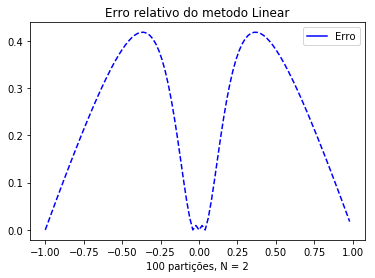
\includegraphics [width=5cm,height=5cm]{ELa2.png}
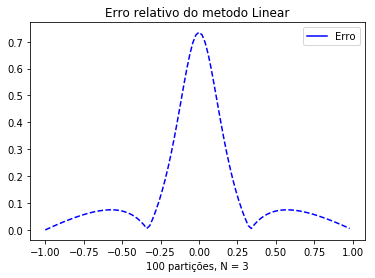
\includegraphics [width=5cm,height=5cm]{ELa3.png}
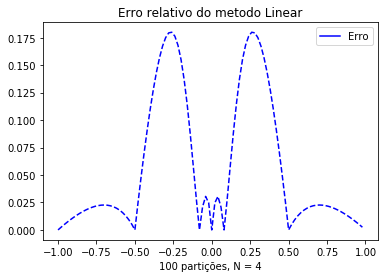
\includegraphics [width=5cm,height=5cm]{ELa4.png}
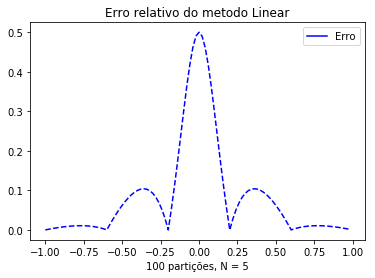
\includegraphics [width=5cm,height=5cm]{ELa5.png}
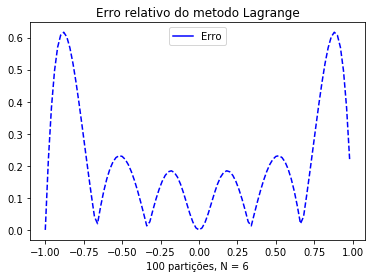
\includegraphics [width=5cm,height=5cm]{ELa6.png}
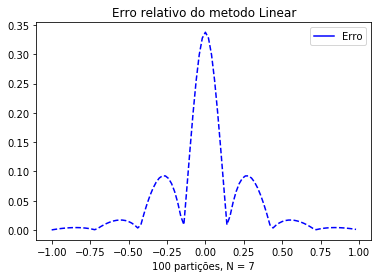
\includegraphics [width=5cm,height=5cm]{ELa7.png}
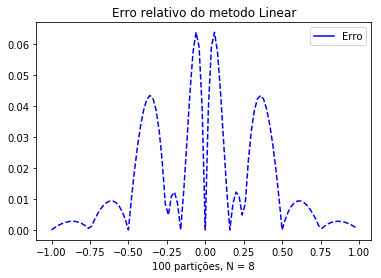
\includegraphics [width=5cm,height=5cm]{ELa8.png}
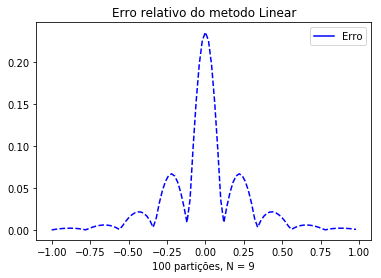
\includegraphics [width=5cm,height=5cm]{ELa9.png}
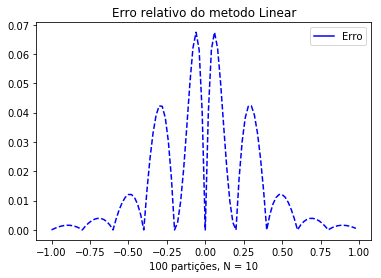
\includegraphics [width=5cm,height=5cm]{ELa10.png}
\end{figure}

\newpage
\text Para a resolução da interpolação do item b:

\begin{figure}[!htb]
\centering
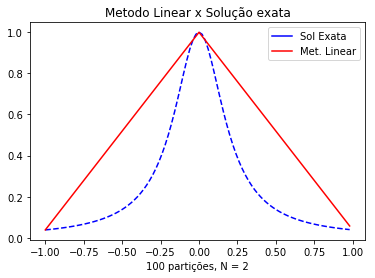
\includegraphics [width=5cm,height=5cm]{LSEb2.png}
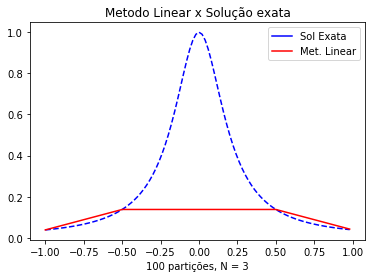
\includegraphics [width=5cm,height=5cm]{LSEb3.png}
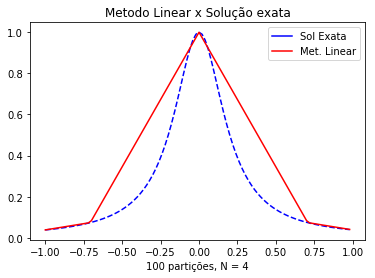
\includegraphics [width=5cm,height=5cm]{LSEb4.png}
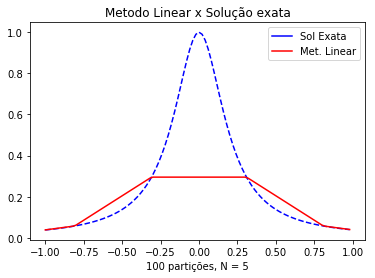
\includegraphics [width=5cm,height=5cm]{LSEb5.png}
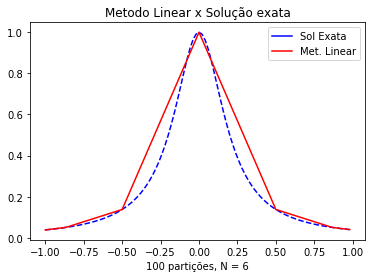
\includegraphics [width=5cm,height=5cm]{LSEb6.png}
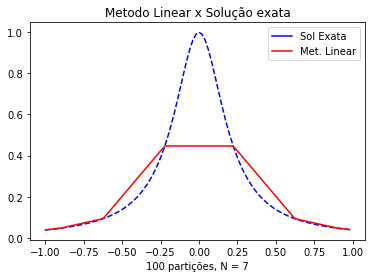
\includegraphics [width=5cm,height=5cm]{LSEb7.png}
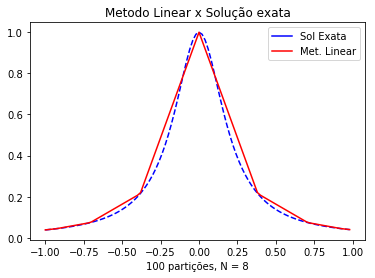
\includegraphics [width=5cm,height=5cm]{LSEb8.png}
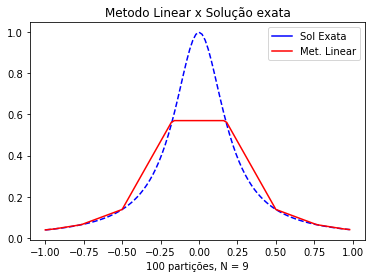
\includegraphics [width=5cm,height=5cm]{LSEb9.png}
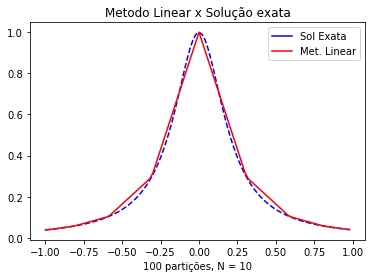
\includegraphics [width=5cm,height=5cm]{LSEb10.png}
\end{figure}

\newpage

\text Seguindo a Solução Exata x O método de Lagrange, temos o erro relativo do método linear de b:

\begin{figure}[!htb]
\centering
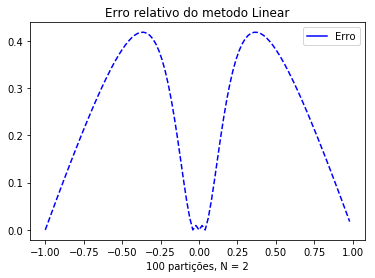
\includegraphics [width=5cm,height=5cm]{ELb2.png}
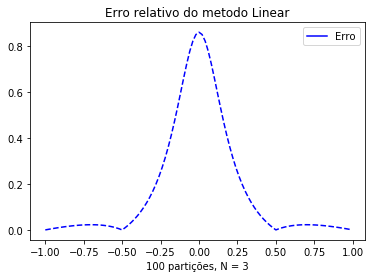
\includegraphics [width=5cm,height=5cm]{ELb3.png}
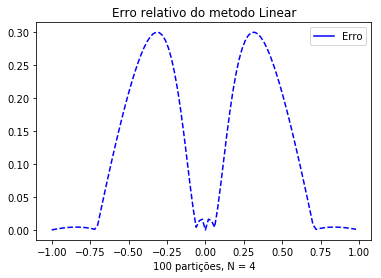
\includegraphics [width=5cm,height=5cm]{ELb4.png}
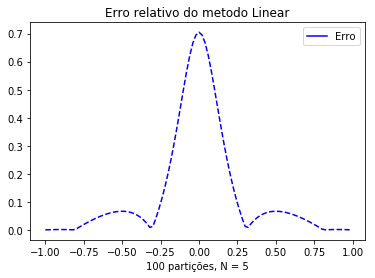
\includegraphics [width=5cm,height=5cm]{ELb5.png}
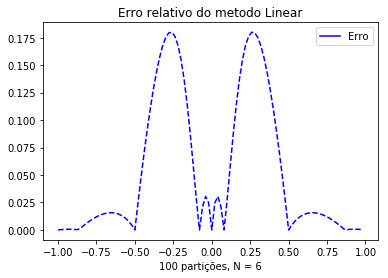
\includegraphics [width=5cm,height=5cm]{ELb6.png}
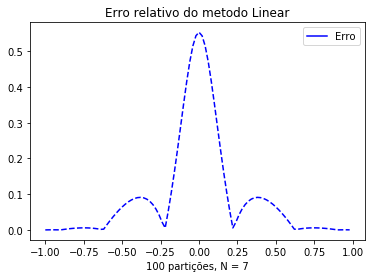
\includegraphics [width=5cm,height=5cm]{ELb7.png}
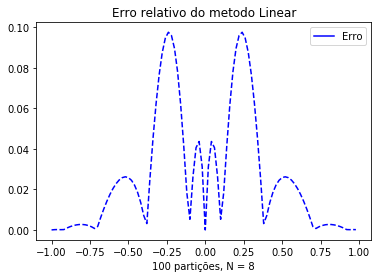
\includegraphics [width=5cm,height=5cm]{ELb8.png}
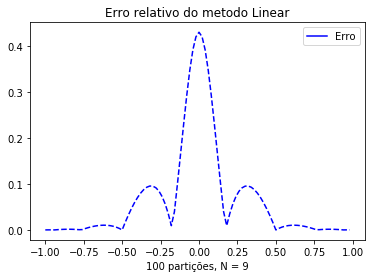
\includegraphics [width=5cm,height=5cm]{ELb9.png}
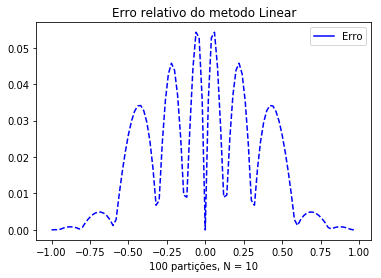
\includegraphics [width=5cm,height=5cm]{ELb10.png}
\end{figure}

\newpage
\text Para a resolução da interpolação do item c:

\begin{figure}[!htb]
\centering
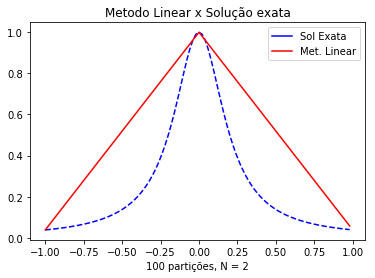
\includegraphics [width=5cm,height=5cm]{LSEc2.png}
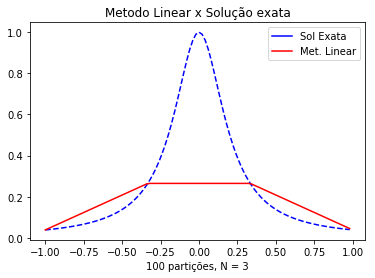
\includegraphics [width=5cm,height=5cm]{LSEc3.png}
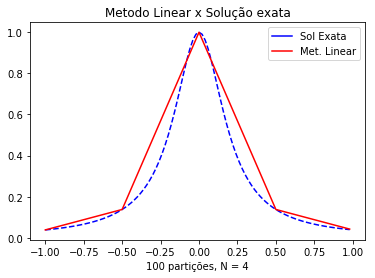
\includegraphics [width=5cm,height=5cm]{LSEc4.png}
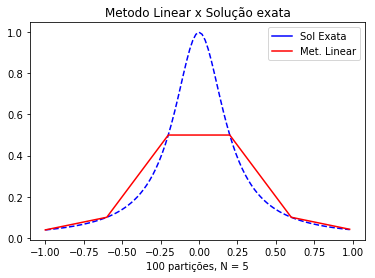
\includegraphics [width=5cm,height=5cm]{LSEc5.png}
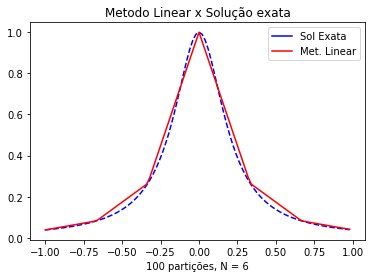
\includegraphics [width=5cm,height=5cm]{LSEc6.png}
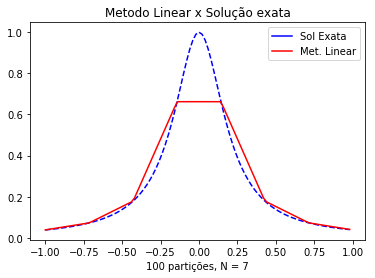
\includegraphics [width=5cm,height=5cm]{LSEc7.png}
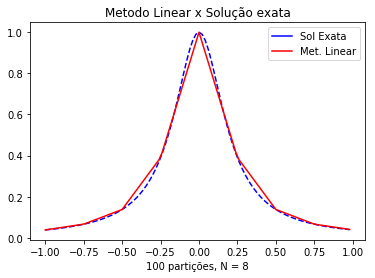
\includegraphics [width=5cm,height=5cm]{LSEc8.png}
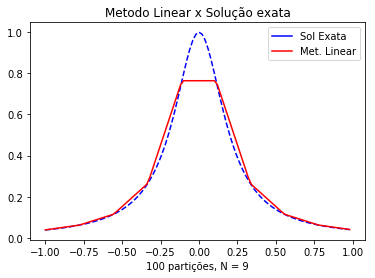
\includegraphics [width=5cm,height=5cm]{LSEc9.png}
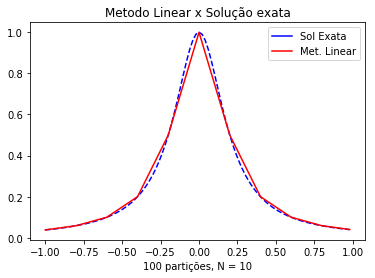
\includegraphics [width=5cm,height=5cm]{LSEc10.png}
\end{figure}

\newpage

\text Seguindo a Solução Exata x O método de Lagrange, temos o erro relativo do método linear de c:

\begin{figure}[!htb]
\centering
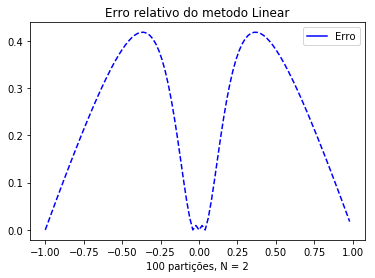
\includegraphics [width=5cm,height=5cm]{ELc2.png}
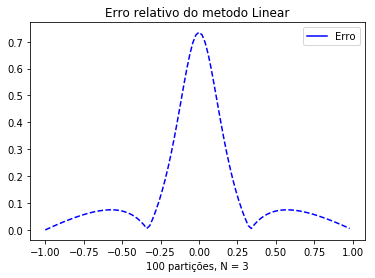
\includegraphics [width=5cm,height=5cm]{ELc3.png}
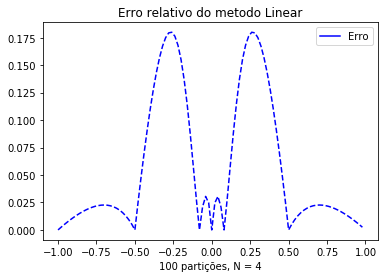
\includegraphics [width=5cm,height=5cm]{ELc4.png}
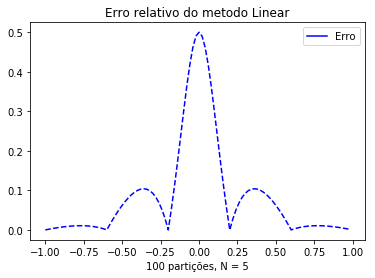
\includegraphics [width=5cm,height=5cm]{ELc5.png}
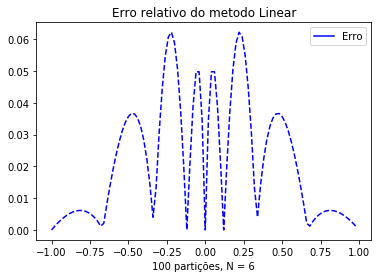
\includegraphics [width=5cm,height=5cm]{ELc6.png}
\includegraphics [width=5cm,height=5cm]{ELc7.png}
\includegraphics [width=5cm,height=5cm]{ELc8.png}
\includegraphics [width=5cm,height=5cm]{ELc9.png}
\includegraphics [width=5cm,height=5cm]{ELc10.png}
\end{figure}


\begin{table}[H!]
\centering
\begin{tabular}{|
>{\columncolor[HTML]{32CB00}}l |
>{\columncolor[HTML]{F8FF00}}l 
>{\columncolor[HTML]{F56B00}}l 
>{\columncolor[HTML]{FE0000}}l }
\hline
\multicolumn{4}{|l|}{\cellcolor[HTML]{32CB00}{\color[HTML]{000000} \textbf{Tabela de Erros}}}                                                             \\ \hline
       & \multicolumn{1}{l|}{\cellcolor[HTML]{F8FF00}a} & \multicolumn{1}{l|}{\cellcolor[HTML]{F8A102}b} & \multicolumn{1}{l|}{\cellcolor[HTML]{FE0000}c} \\ \hline
n = 2  & {\color[HTML]{000000} }    
    0.4179970972423803
   &            0.6461538461538463            &        0.4179970972423803 \\ \cline{1-1}
n = 5  & {\color[HTML]{F8FF00} }    0.4999999999999999        &    0.7047785346705744  &  0.4999999999999999  \\ \cline{1-1}
n = 10 & {\color[HTML]{F8FF00} }     0.06743119266055053    &   0.05427386749715091  &   0.4999999999999999  \\ \cline{1-1}
\end{tabular}
\caption{Tabela do erro máximo de interpolação para n = 2,5 e 10}
\end{table}

\text Comparando o resultado dos métodos, observamos uma aproximação do erro para determinadas funções e uma diferença em outras.  Para as funções de "a" e de "c" o erro é o mesmo em determinados momentos e em outros ele se afasta consideravelmente; "b" é a função com resultados mais discrepantes das outras funções.

\end{document}
